% !TeX spellcheck = en_US
\documentclass[11pt, fleqn, titlepage]{article}
%\usepackage{siunitx}
\usepackage{texfiles/SpeedyGonzales}
\usepackage{texfiles/MediocreMike}
\newcommand{\so}[2]{{#1}\mathrm{e}{#2}}
% \geometry{top=1cm}
\usepackage{hyperref}
\usepackage{amsmath}
\usepackage{ragged2e}
\usepackage{booktabs}
\usepackage{lipsum}
\hypersetup{
	colorlinks=true,
	linkcolor=blue,
	filecolor=magenta,      
	urlcolor=cyan,
}
\usepackage{subfig}
\usepackage{graphicx}
\title{Fairness in Classification}
\author{Anders Henriksen \\ Oskar Eiler Wiese Christensen  \\ \texttt{\{s183917, s183904\}@student.dtu.dk}}
\date{\today}

\pagestyle{plain}
\fancyhf{}
\rfoot{Page \thepage{} of \pageref{LastPage}}

\graphicspath{{Billeder/}}

\begin{document}
	
	\maketitle
	\begin{abstract}
		\textbf{TODO: Skal indeholde motivation, problem, fremgangsmåde, resultater og konklusion.} \\ \lipsum[1-2]
	\end{abstract}
	\tableofcontents \newpage
	%\thispagestyle{fancy}
	%\tableofcontents	
	
	\section{Abstract}
	\textbf{TODO: Skal indeholde motivation, problem, fremgangsmåde, resultater og konklusion.}
	
	\section{Introduction}
	\textbf{TODO: \\ Hvad er formålet med projektet? \\ Hvad er problemformuleringen \\ Hvad er state-of-the-art? \\ Hvilken fremgangsmåde bruges til at løse problemet? \\ Hvem har brug for resultaterne?}
	
	\subsection{Motivation}
	Artifical intelligence (AI) and machine learning (ML) methods are playing a bigger and bigger role in modern society. As the accuracies of AI and ML models increase, their applications become wider, allowing for these  models to be implemented either as ground truth or as a pointer in applications like autonomous vehicles, medical imaging, the American judicial system. These models are, for the general public, often seen as an objective decision maker. As such, it becomes of essence to avoid discrimination, since discrimination in models could lead to reinforced societal discrimination. A saving grace in this case would be to implement bias correction on either the dataset or the model, thereby removing the risk of discrimination. In that sense, it also becomes important to examine whether
	
	\begin{enumerate}
		\item How is the data "crooked" in the data-set used by the COMPAS algorithm? What bias exists in the data?
		\begin{itemize}
			\item[i)] How do we analyse whether there is bias in the data and which kind of bias there is? 
			\item[ii)] What does it mean that there is a bias in the data?
		\end{itemize}
		
		\item How does bias in the data affect a classification algorithm?
		\begin{itemize}
			\item[i)] What does it mean that an algorithm is biased?
			\item[ii)] How do we quantify that there is in fact a bias in the algorithm?
		\end{itemize}
		
		\item Understand and implement a bias-correction method from the paper "Equality of Opportunity in Supervised Learning". 
		%	\begin{itemize}
		%		\item[i)] If time allows for it, other bias correction methods will be taken into consideration and evaluated.
		%	\end{itemize}
		
		\item Which applications can bias-correction algorithms as well as AI-models have in society? And how can society gain trust in these models? 
	\end{enumerate}
	
	\subsection{State of the Art}
	
	
	\subsection{Contributions}

	
	
	\section{Data}
	\textbf{TODO: \\ Data kan kort introduceres i indledningen \\ Lav etisk diskussion om opbevaring af data samt privacy issues}
	
	\subsection{Description of Data}
	The data used in this project stems from an initial analysis of the COMPAS (Correctional Offender Management Profiling for Alternative Sanctions) algorithm by its developers, Northpointe Inc. After this analysis, ProPublica made a subsequent analysis of this data as well as their own queries of the offenders involved and data of the offenders who actually recidivated. This data is stored in the \texttt{compas-scores-two-year.csv} dataset from ProPublica's GitHub page, which can be found here: \url{https://github.com/propublica/compas-analysis/blob/master/compas-scores-two-years.csv}. \\\\
	\noindent The data consists of 53 different variables, 9 of which are used in the binary classification model. Four of the chosen variables are categorical, so these will have to be one-out-of-k encoded to be able to feed the necessary variables into the neural network. Meanwhile, the numerical variables, of which there are also four, will be normalized as to avoid the vanishing gradient problem and to avoid having some variables be of more importance to the final prediction. This will be explained more thoroughly in \ref{Feed-forward neural}. \\
	The 10 chosen variables, of which one will be used as the target variable are shown and explained below.
	
	
	\begin{table}[H]\label{resultater}
		\centering
		\begin{tabular}{l l l}
			Variable & Description & Type \\ \hline
			age & The age of the offenders & Continuous ratio \\
			priors\_count & The number of previous offences & Discrete interval \\
			juv\_fel\_count & The number of previous juvenile felonies & Discrete interval \\
			juv\_misd\_count & The number of previous juvenile misdemeanor & Discrete interval \\
			c\_charge\_degree & The severity of the offence & Discrete nominal \\
			race & The race of the offender & Discrete nominal \\
			age\_cat & The age category of the offender & Discrete nominal \\
			sex & The sex of the offender & Discrete nominal \\
			score\_text & The COMPAS prediction of chance of recidivism & Discrete interval
		\end{tabular}
		%\caption{text}
	\end{table}
		
		
	\subsection{Visualization of Data}
	To better get an understanding of the data, a range of plots are shown below. \ref{fig:predictedrecidrace} aims to show wheter there is a difference between the fraction of whites and african-americans that are predicted by the COMPAS classifier as having low, medium and high risk of recidivism. \ref{fig:predictedrecidsex} has the same purpose, utilizing sex instead of race. \ref{fig:truerecid} and \ref{fig:proirs} give some insight into the actual amount of crime done by african-americans and whites and whether the amounts seem to be similar.
	
	\begin{figure}[H]
		\centering
		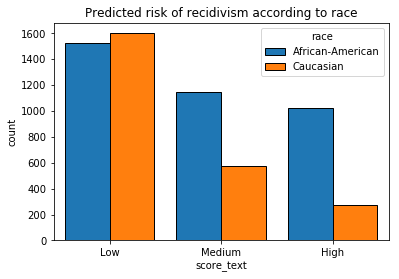
\includegraphics[width=0.5\linewidth]{imgs/predicted_recid_race}
		\caption{It is clear from this illustration that the number of caucasian and african-american people in the low group are almost equal. Meanwhile the medium and high groups contain a much larger fraction of african-americans. Since, in total, there are more african-americans in the dataset than whites (3696/2454), it would seem based purely on the data that whites are more often classified as low risk of recidivism while african-americans are often classified as medium or high risk.}
		\label{fig:predictedrecidrace}
	\end{figure}
	
	\begin{figure}[H]
		\centering
		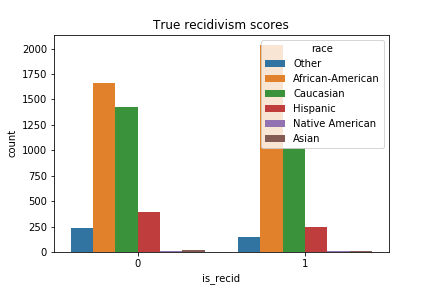
\includegraphics[width=0.5\linewidth]{imgs/true_recid}
		\caption{This illustration shows the true recidivism values (0 being no recidivism after two years and 1 being recidivism) for all offenders in the dataset seperated by the race of each offender. It is clear that close to an equal amount of white and african-american offenders did not recidivate, while a much larger proportion of african-americans re-offended than whites. This makes it difficult to prove bias in the data based only on the data, as it is not necessarily a bias that african-americans more often re-offend.}
		\label{fig:truerecid}
	\end{figure}
	
	\begin{figure}[H]
		\centering
		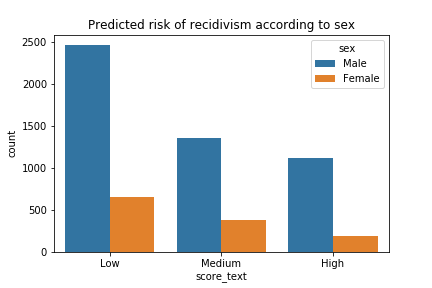
\includegraphics[width=0.5\linewidth]{imgs/predicted_recid_sex}
		\caption{This illustration shows the relationship between sex and the COMPAS prediction of recidivism. The first point to be noted is that there are a lot more men in the dataset than women (5819/1395). Aside from this, it does not seem like there is a difference in the proportions of men or women being classified as belonging to each of the categories.}
		\label{fig:predictedrecidsex}
	\end{figure}
	
	\begin{figure}[H]
		\centering
		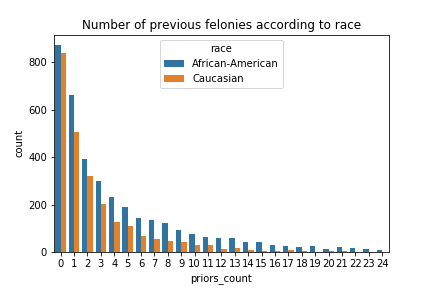
\includegraphics[width=0.5\linewidth]{imgs/proirs}
		\caption{An illustration of the relation between race (african-american or caucasian) and the number of previous felonies prior to the study taking place. This plot gives a clear indication that the number of whites and african-americans who have performed no prior felonies is similar. Otherwise, it is clear that the proportion of african-american to whites becomes larger as the number of previous felonies becomes larger. This seems to indicate that african-americans are more often engaged in criminal activity, which also weakens the indication of a bias from \ref{fig:predictedrecidrace}.}
		\label{fig:proirs}
	\end{figure}
	
	
	
	\subsection{Bias in Data}
	
	
	\section{Methods}
	\textbf{TODO: \\ referér til kode og software \\ brug lang tid på nye metoder, kort tid på gamle metoder}
	
	\subsection{Binary Classifier}\label{Feed-forward neural}
	%initialization schemes
	\subsubsection{Feed-forward Neural Network}
	Feed-forward neural networks (FFNN) are the simplest form of a neural network. Information flow in a feed-forward neural is one directional which means that the network has an input layer, and information flow from these nodes through the hidden layers unto the output layer. The main purpose of a FFNN is to approximate a function. In this project $ y = f^*(x) $ maps an input $ \mathbf x $ to a category $ \mathbf y $. The FFNN is thereby a classifier, which goal is to determine the recidvism risk of a person given the input variable $ \mathbf x $. The input variable $ \mathbf x $ contains :::::. The categories of $ \mathbf y $ is either 0 or 1, which corresponds to the classifier classifying a person as either low or medium/high risk of recidivism. Hence, this is a binary classifier which constructs a mapping $ \mathbf y = f(\mathbf x \ ; \mathbf w) $. The goal is to learn the weights that most efficiently approximate the function $ f^* $ through supervised learning. The binary classifier in this project has an input layer, three hidden layers and an output layer. 
	
	\begin{figure}[H]
		\centering
		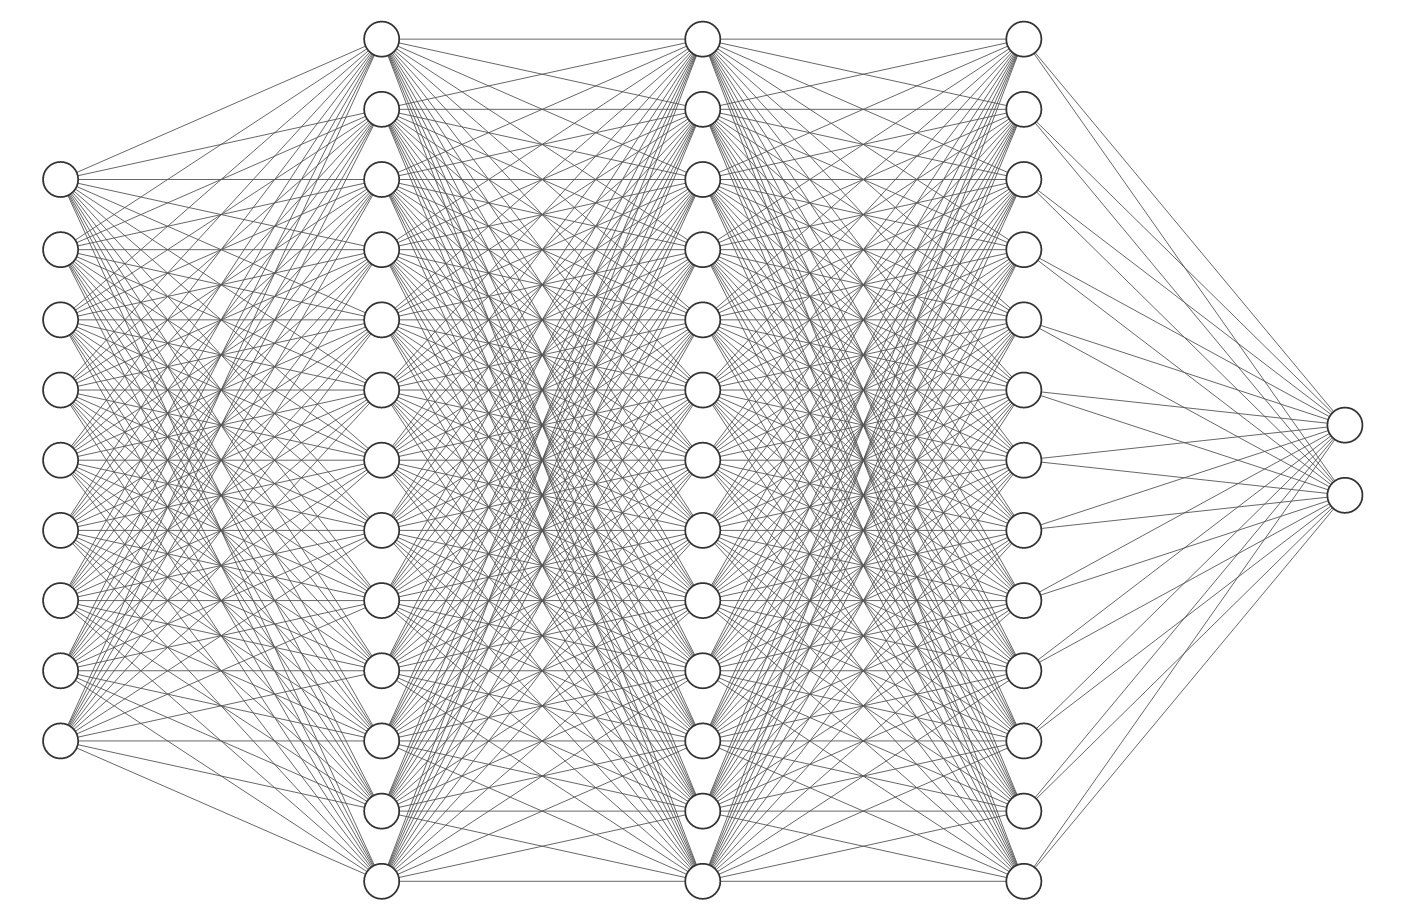
\includegraphics[width=0.5\linewidth]{imgs/ffnn}
		\caption{Visualization of the binary classifier model. The input layer has dimension $ \mathbb R ^9$ and the output layer has dimension $ \mathbb R^2 $. The number of nodes in the hidden layers is a changeable parameter which is found with Bayesian Optimization. }
		\label{fig:ffnn}
	\end{figure}
	
	
	\subsubsection{Bayesian Optimization}
	%Bayesian Optimization
	
	To obtain the pinnacle of accuracy in a neural network, it needs an excellent architecture as well as the potimal hyperparameters. However, the search for these parameters are usually a costly process of uncertainty balancing exploration of parameters and the exploitation of results. Often the process of finding the optimal parameters and network architecture comes from expert knowledge, biased heuristics or exhaustive sampling from the parameter space. To determine the architecture and hyperparameters of the binary classifier Bayesian Optimization is used. 
	\subparagraph*{Objective Function}
	The objective function that is being optimized in this project is the binary classifier presented above. The fully connected layers are trained on the COMPASS data-set and the validation accuracy of the model is what BO optimizes. The accuracy of the constructed model is evaluated using non-parametric Gaussian Process (GP) as a function fo the following hyperparameters:
	\begin{itemize}
		\item Number of units in the first hidden layer \(\in [1, 5000]\) 
		\item Number of units in the second hidden layer \(\in [1, 5000]\) 
		\item Number of units in the third hidden layer \(\in [1, 5000]\)
		\item Dropout probability \(\in [0,1]\)
		\item Activation function \{tanh, ReLU, ReLU6, Sigmoid\}
	\end{itemize}
	The hyperparameters that are not changed are the learning rate, which is set at $ \alpha = 0.001 $. The reason why this parameter is not changed is due to the fact, that the optimizer implemented in this project, is Adaptive Moment Estimation (Adam). Adam is a well known optimizer in the literature and has adaptive learning rate as well as step size. Which is why this learning rate is not an interchangeable hyperparameter. \\ Cross Entropy Loss is used as the cost-function. \textbf{TODO: skriv noget om funktionen. }
	\\\\
	Gaussian Process uses the smoothness assumption on the outputs of the network, and its variance and lengthscale parameters are optimized using maximum log-likelihood principle. \cite{aktiv_gp} The acquisition function, that choose the parameters for the model, used is Expected Improvement (EI). EI attempts to quantify the improvement of the parameters chosen. The average improvement is quantified by sampling the objective function at $x$. The acquisition function then computes the expected value of the improvement function at a certain $x$. EI is expressed as 
	\begin{equation*}
	\mathrm{EI}(\mathbf{x})=\left\{\begin{array}{ll}
	\left(\mu(\mathbf{x})-f\left(\mathbf{x}^{+}\right)\right) \Phi(Z)+\sigma(\mathbf{x}) \phi(Z) & \text { if } \sigma(\mathbf{x})>0 \\
	0 & \text { if } \sigma(\mathbf{x})<0,
	\end{array}\right. 
	\end{equation*}
	where $ Z = \frac{\mu(\mathbf{x}) - f(\mathbf{x}^+) - \xi }{\sigma(\mathbf{x})}$ , \cite{aktiv_bo} 
	\\\\
	The Bayesian Optimization starts by sampling from the objective function, then it fits the Gaussian Process to the sampled points and then iterates the next points in the hyperparameter space using the fitted GP and Expected Improvement. As for the implementation of Baysesian Optimization the GPyOpt library is used \cite{bo_lib}. The exploration / exploitation trade-off variable \textit{jitter} is set to the default value of 0.01.
	
	\subsection{Permutation test}
	
	
	\subsection{Bias Correction	n Methods}
	
	\section{Results}
	\textbf{TODO \\ dokumentér reproducerbarheden af resultaterne \\ tabeller og figurer over resultater \\ forklar resultaterne endten i diskussion eller resultater.}
	
	\section{Discussion}
	\textbf{TODO: \\ etisk diskussion omkring teknologien der er arbejdet med}
	
	\section{Conclusion}
	\textbf{TODO: \\ Opsummér resultater og anbefalinger fra projektet \\ Må ikke indeholde noget nyt \\ Skal svare på spørgsmålene fra problemformuleringen \\ Konklusion, abstract og indledning skal give samlet billede af projektet}
	
	\section{Appendix}
	
	\begin{figure}[H]
		\centering
		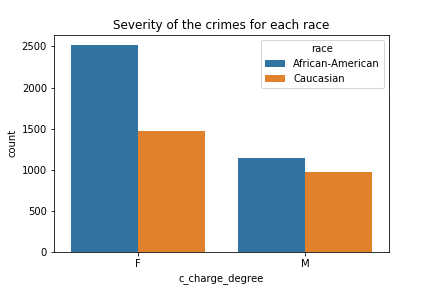
\includegraphics[width=0.5\linewidth]{imgs/c_charge_degree}
		\caption{}
		\label{fig:cchargedegree}
	\end{figure}
	
	\begin{figure}[H]
		\centering
		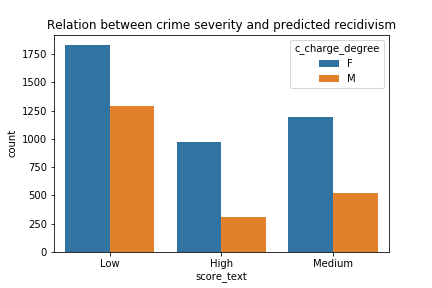
\includegraphics[width=0.5\linewidth]{imgs/charge_degree_score}
		\caption{}
		\label{fig:chargedegreescore}
	\end{figure}
	
	\begin{thebibliography}{9}
		
		\bibitem{bo_lib} Machine Learning Group, University of Sheffield: "GPyOpt’s documentation", at \url{https://gpyopt.readthedocs.io}
		
		\bibitem{aktiv_gp} 
		
		\bibitem{aktiv_bo} 
		
	\end{thebibliography}
	
	\newpage
	\bibliographystyle{IEEEbib}
	\bibliography{refs}
\end{document}
